\section{The worst case at a given sample size}\label{sec:worst}

The results so far take one law at a time. A user who does not know the law faces the worst-case size $S_n(\alpha)$ of \cref{sec:setting}, in which the worst law may change with $n$. Such moving laws can sit between the cases that \cref{thm:upper} handles: a shoulder whose height approaches that of the top at rate $n^{-1/2}$, two flat blocks that merge, or a shoulder that shrinks as $n$ grows. This section shows that moving laws do no worse in the limit than the fixed shoulders of \cref{sec:mechanism}. The argument reduces every law to a uniform sample, then reduces the large-sample problem to a question about one Brownian bridge, and answers that question by computation.

\subsection{Reduction to uniform samples}
The reduction uses three objects. The first is a set of fits with a fixed turning point: for $u\in[0,1]$, $K_u$ is the set of continuous functions on $[0,1]$ that are convex on $[0,u]$ and concave on $[u,1]$. The second is the distance to that set, written $d(h,K_u)$ and measured in the supremum norm. The third is the data sent through their own distribution function: the variables $U_i=F(X_i)$ are uniform, $\Gamma_n$ is their empirical distribution function, and $u=F(m)$ is where the mode lands on this probability scale.

\begin{theorem}[domination]\label{thm:envelope}
Let $F$ be continuous unimodal with mode $m$, put $u=F(m)$, and let $\Gamma_n$ be the empirical distribution function of the uniform variables $U_i=F(X_i)$. Then for every sample
\[
D(F_n)\ \le\ d(\Gamma_n,K_u).
\]
\end{theorem}

To see this, let $\varphi\in K_u$ fit the uniform sample within distance $e$. Make $\varphi$ constant to the left of its minimum on $[0,u]$ and to the right of its maximum on $[u,1]$. The result is nondecreasing, still belongs to $K_u$, and is still within $e$ of $\Gamma_n$, because $\Gamma_n$ is nondecreasing. Composing with $F$ then gives a unimodal fit to the original sample: a nondecreasing convex function of a convex function is convex, so the composition is convex up to $m$, and the same argument makes it concave after $m$. Its error is still $e$, because $F_n=\Gamma_n\circ F$. So the original sample is never further from unimodality than the uniform sample is from $K_u$.

The theorem says that, at every $n$, the worst null law is no worse than a uniform sample whose fit is forced to turn at some point $u$. Reflecting the data, $x\mapsto-x$, keeps the dip, exchanges convex and concave, and sends $u$ to $1-u$, so we may take $u\ge\frac12$. For the running example the mode is the top interval, so $u$ can be any point of $[0.9,1]$. Two consequences follow. First, the worst-case size depends on the unknown law only through one number, $u$, so it can be bounded by checking uniform samples at all turning points. \Cref{sec:finite} does this with exact linear programs. Second, $u=1$ forces a convex fit everywhere, which is the full-mass shoulder of \cref{sec:mechanism}. The question becomes whether any other turning point is worse.

\subsection{Reduction to one Brownian bridge}
As $n$ grows, $\sqrt n(\Gamma_n-\mathrm{id})$ converges in distribution to a Brownian bridge. Adding a linear function to a member of $K_u$ gives another member, so subtracting the identity does not change the distance, and $\sqrt n\,d(\Gamma_n,K_u)$ converges to $d(B,K_u)$. Let
\[
g(u,t)=P\bigl(d(B,K_u)\ge t\bigr)
\]
be the probability that a Brownian bridge is at least $t$ away from every function turning at $u$. We call $u=1$ the \emph{edge}: there $K_1$ is the set of convex functions, so $g(1,t)=1-F_M(2t)$ by \cref{lem:halfgap}. The next theorem says that the worst law at large $n$ lies between the edge value and the worst turning point.

\begin{theorem}[Brownian reduction]\label{thm:reduction}
For every $t>0$,
\[
P(M/2>t)\ \le\ \liminf_{n\to\infty}\,\sup_F P_F(\sqrt nD_n>t)\ \le\ \limsup_{n\to\infty}\,\sup_F P_F(\sqrt nD_n>t)\ \le\ \sup_{u\in[1/2,1]}g(u,t),
\]
where the suprema run over all continuous unimodal laws.
\end{theorem}

The lower bound is \cref{thm:shoulder}. For the upper bound, \cref{thm:envelope} replaces every law by a uniform sample, and a strong approximation couples the uniform empirical process with Brownian bridges \cite{KMT75}. The remaining difficulty is to make the approximation hold for all turning points at once. We split the bridge at $u$ into two independent bridges, one on each side (\cref{lem:seam}), which makes $d(B,K_u)$ continuous in $u$ under a single coupling; and $d(B,K_u)$ has no atom at any $t>0$, because it is a convex functional of a Gaussian process. A compactness argument then gives the uniform statement. The full proof is in \cref{app:proofs}.

If the edge were always the worst turning point, that is $g(u,t)\le g(1,t)$ for every $u$, the two ends of \cref{thm:reduction} would meet at $1-F_M(2t)$, and the worst case over all laws would be the flat shoulder of \cref{sec:mechanism}.

\subsection{Why the edge should be the worst turning point}
Moving the turning point a little way in from the edge changes two things, and they pull in opposite directions. Put the turning point at $u=1-\varepsilon^2$ with $\varepsilon$ small. On the long left side, of probability length $u$, the fit must still be convex, but this side is now slightly shorter than the whole interval, so its convex distance is $\sqrt u$ times a copy of $M/2$ instead of $M/2$ itself, and the probability of exceeding $t$ falls. To first order the loss is $\varepsilon^2\,t\,f_M(2t)$, where $f_M$ is the density of $M$. On the short right side, of length $\varepsilon^2$, the fit may now bend downward, and where the two sides meet (the seam) the fit gains a little extra room. The gain in exceedance probability is at most about $\varepsilon^2 f_M(2t)/(4t)$. Comparing the two, the loss is larger whenever $t>\frac12$, so for such $t$ the edge is a strict local maximum of $g(\cdot,t)$; in symbols,
\[
g(1-\varepsilon^2,t)\ \le\ g(1,t)-\varepsilon^2f_M(2t)\Bigl(t-\frac1{4t}\Bigr)+o(\varepsilon^2)\qquad(t>\tfrac12).
\]
We have a written proof of this expansion, given in the supplementary notes; it is not used in the rest of the paper. It explains the shape of the problem, but it does not settle it for two reasons. It says nothing about turning points far from the edge, and the cutoffs of the standard test lie close to $\frac12$ (between about $0.49$ and $0.64$), where the margin $t-1/(4t)$ is small or even negative.

\subsection{Checking the edge at the standard cutoffs}
The standard test uses the cutoff $\qbar_\alpha$, which we know only within its certified bracket. We therefore work at a value $t'$ just below the lower end of that bracket. Because $t'<\qbar_\alpha$, every rejection by the standard test eventually has $\sqrt nD_n>t'$, so an upper bound at $t'$ is an upper bound for the standard test. At the 5 percent level, for example, $t'=0.5378$ and the edge value $g(1,t')=1-F_M(2t')$ is $33.2$ percent, the upper end of the interval in \cref{tab:size}. The task is to show that no other turning point exceeds the edge at $t'$.

\begin{figure}[t]
\centering
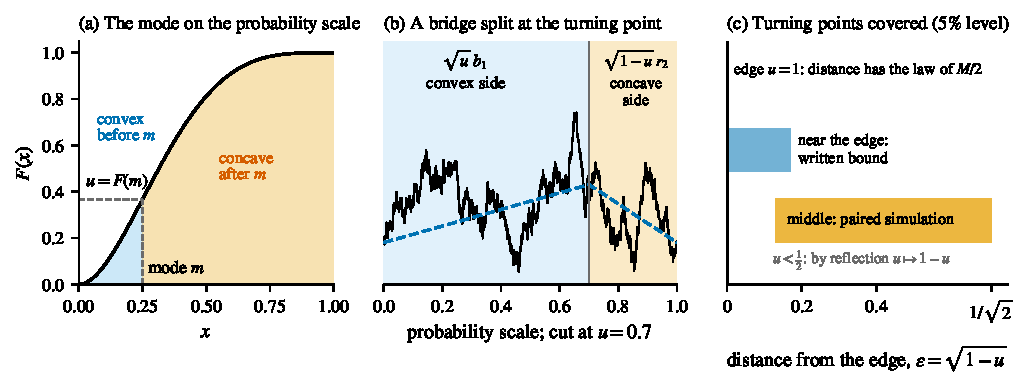
\includegraphics[width=\linewidth]{figs/fig7_dependency.pdf}
\caption{The geometry behind \cref{sec:worst}: every law reduces to a uniform sample with a fixed turning point, the bridge splits there into two independent halves, and two arguments together cover every turning point. (a) A unimodal distribution function curves upward before the mode $m$ and downward after it; on the probability scale the mode sits at $u=F(m)$. (b) One simulated Brownian bridge cut at $u=0.7$: after the dashed broken line is removed, the left piece is $\sqrt u\,b_1$ and the right piece is $\sqrt{1-u}\,r_2$, two independent bridges (\cref{lem:seam}); the fit must be convex on the left and concave on the right. (c) At the 5 percent level, the turning points near the edge are handled by a written bound and those in the middle by a paired simulation; the two ranges overlap, the edge itself gives the law of $M/2$, and reflection covers $u<\frac12$.}
\label{fig:dependency}
\end{figure}

We split the turning points into two overlapping ranges, as \cref{fig:dependency}(c) shows. Close to the edge, the two pieces of the bridge in \cref{lem:seam} are very unequal: the right piece is short, of scale $\varepsilon=\sqrt{1-u}$. There a written argument bounds $g(u,t')-g(1,t')$ from above by an explicit expression in published laws of Brownian functionals, including the description of the convex minorant of Brownian motion by Pitman and Uribe Bravo \cite{PUB12}, and interval arithmetic shows that the expression is negative throughout that range. Further from the edge no such expansion is accurate, and we compare each turning point directly with the edge on the same simulated pairs of bridges. For each pair we record whether the edge exceeds $t'$ while no turning point in a small cell does, or the reverse; the record is built so that its expected value is at least the largest rejection probability in the cell minus the one at the edge, so a negative expectation covers every turning point in the cell, not only a grid of them. A sign test in each cell shows that the edge wins by a wide margin. Reflection, $u\mapsto1-u$, covers turning points left of the middle.

The exact ranges, the number of cells and paths, and the error budget are listed in \cref{app:cert}. The probability that the two computations together certify a false statement is at most $1.1\cdot10^{-3}$ at each level.

\begin{theorem}[worst-case size; certified, conditional]\label{thm:worst}
Assume the quantile convergence of \cref{sec:setting}, the written lemmas behind \cref{thm:reduction} (\cref{lem:seam} and the proof in \cref{app:proofs}), and the four written lemmas behind the near-edge bound (\cref{app:cert}). On the event that the two certificates above and the bracket for $\qbar_\alpha$ are correct, both $\liminf_nS_n(\alpha)$ and $\limsup_nS_n(\alpha)$ lie in
\[
[40.45,\,46.22]\%\ \ (\alpha=10\%),\qquad[28.40,\,33.20]\%\ \ (\alpha=5\%),\qquad[12.67,\,16.79]\%\ \ (\alpha=1\%).
\]
\end{theorem}
\begin{proof}
Because $t'<\qbar_\alpha$, the uniform critical values satisfy $\sqrt n\,q_n(1-\alpha)>t'$ for all large $n$, so rejection implies $\sqrt nD_n>t'$. \Cref{thm:reduction} and the certified edge statement then give $\limsup_nS_n\le g(1,t')=1-F_M(2t')$. For the lower bound, $S_n$ is at least the rejection probability of any fixed law, so \cref{cor:lf}(b) gives $\liminf_nS_n\ge1-F_M(2\qbar_\alpha)\ge1-F_M(2q_+)$. The rigorous enclosure of $F_M$ turns both ends into the numbers shown.
\end{proof}

These intervals are the ones in \cref{tab:size} for fixed laws; we do not show that the two quantities are equal, only that both lie in the same intervals. Moving laws do not make the standard test worse in the limit by more than the width of these intervals, and the flat shoulder with a thin top comes within that width of the worst case. We do not claim that $\lim_nS_n$ exists, or that any law attains it.

The same machinery answers whether $c_\alpha$ also controls the worst-case size. At $t=c_\alpha$ an analogous computation certified, with joint confidence at least $0.99$, that $g(u,c_\alpha)<\alpha$ for $u\in[0.0159,0.9841]$ at 5 percent and $u\in[0.0176,0.9824]$ at 1 percent. A written near-edge theorem, checked in Lean given its published inputs, covers $u\in[0.9775,1)$. On the event that the certificate is correct, and conditional on the same lemmas, $\lim_n\sup_FP_F(\sqrt nD_n>c_\alpha)=\alpha$ at both levels: the corrected cutoff keeps its level uniformly over all continuous unimodal laws, in the limit.
